\documentclass{beamer}
\usetheme{Warsaw}

\usepackage[utf8]{inputenc}
\usepackage{fancybox}
\usepackage{multimedia} 
\usepackage{subfig}
\usepackage{amsmath}
\usepackage{hyperref}
\usepackage[all]{xy}
\usepackage{algorithm}
%\usepackage{arevmath}     % For math symbols
\usepackage[noend]{algpseudocode}

\begin{document}



\title[Stochastik] % (optional, only for long titles)
{Stochastik für Informatiker
\\
\includegraphics[scale=0.5]{img/craps}
}
\subtitle{}
\author[Dr. Johannes Riesterer] % (optional, for multiple authors)
{Dr.  rer. nat. Johannes Riesterer}

\date[KPT 2004] % (optional)
{}

\subject{Stochastik}







\begin{frame}
    \frametitle{Stochastik}
\framesubtitle{Lebesgue Maß}
    \begin{block}{Wie kann man Inhalte messen?}
Archimedes approximierte den Flächeninhalt einer Kreisscheibe durch Vielecke, deren Flächeninhalt man leicht berechnen kann (250 v. Chr.).
\begin{align*}
\frac{223}{71} < \pi < \frac{22}{7}
\end{align*}
\begin{figure}[H]
      \centering
    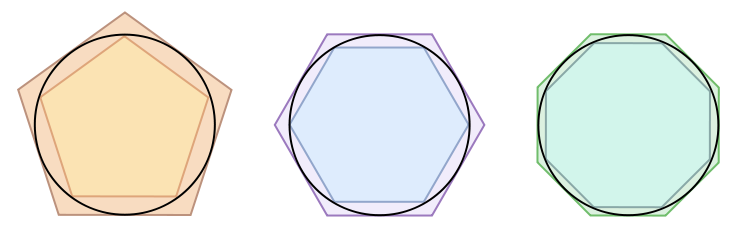
\includegraphics[width=0.7 \textwidth]{img/750px-Archimedes_pi}
      \caption{Quelle: Wikipedia: https://en.wikipedia.org/wiki/File:Archimedes\_pi.svg}
\end{figure}
\end{block}
 \end{frame}



\begin{frame}
    \frametitle{Stochastik}
\framesubtitle{Lebesgue Maß}
    \begin{block}{Idee}
\begin{itemize}
\item Überdecke komplizierte Mengen mit einfachen Mengen, deren Inhalt man leicht berechnen kann.
\item \pause Mit Hilfe eines Grenzwertprozesses konstruiert man eine beliebig genaue Überdeckung.
\end{itemize}
\end{block}
\begin{figure}[!tbp]
  \centering
  \begin{minipage}[b]{0.4\textwidth}
    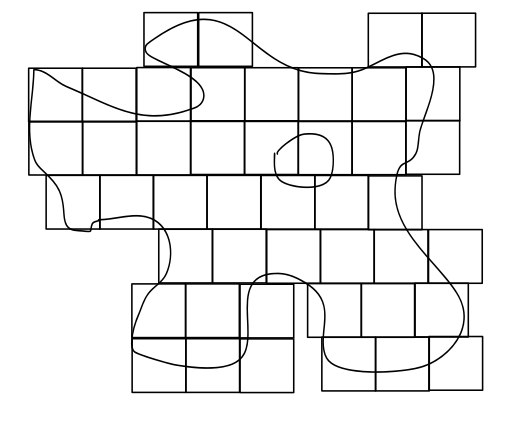
\includegraphics[width=\textwidth]{img/leb1-2}
    \caption{Grobe Überdeckung}
  \end{minipage}
  \hfill
  \begin{minipage}[b]{0.4\textwidth}
    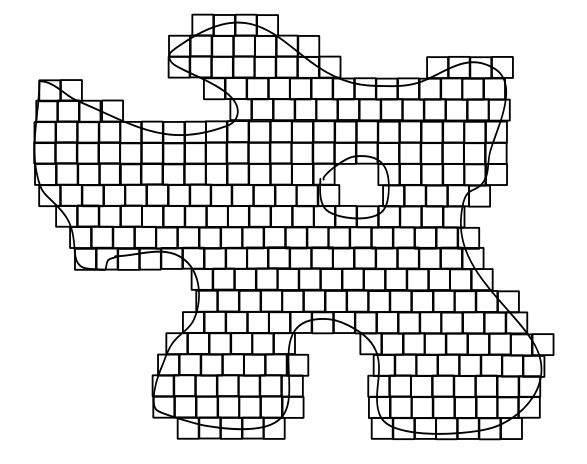
\includegraphics[width=\textwidth]{img/leb2-11}
    \caption{Feinere Überdeckung}
  \end{minipage}
\end{figure}
 \end{frame}





\begin{frame}
    \frametitle{Stochastik}
\framesubtitle{Lebesgue Maß}
    \begin{block}{Quader}
Für abgeschlossene Intervalle $[a_i,b_i] \subset \mathbb{R}$ mit $a_i \leq b_i$ nennen wir 
$$I := [a_1,b_1] \times \cdots \times [a_n,b_n]$$ 
einen $n$-dimensionalen Quader und 
$$\overset{\circ}{I}:= [a_1, b_1] \times \cdots \times [a_n,b_n]$$
 sein Inneres. Wir definieren das Volumen 
\begin{align*}
\text{vol} (I):=   \prod_{i = 1}^n (b_i -a_i)  \; .
\end{align*}

\end{block}
 \end{frame}



\begin{frame}
    \frametitle{Stochastik}
\framesubtitle{Lebesgue Maß}
    \begin{block}{Quader}
Mit $$\mathbb{I}(n): = \{   [a_1,b_1] \times \cdots \times [a_n,b_n] \; | \;  [a_i, b_i] \subset \mathbb{R} \}$$ bezeichnen wir die Menge aller $n$-dimensionalen Quader. 
\end{block}
    \begin{block}{Degenerierte Quader}
Mit $$\mathbb{I}^0(n): = \{   [a_1,b_1] \times \cdots \times [a_n,b_n] \; | \;  [a_i, b_i] \subset \mathbb{R}  \text { und } a_k = b_k \text{ für ein k}\}$$ bezeichnen wir die Menge aller $n$-dimensionalen degenerierten Quader. 
\end{block}
 
 \end{frame}


 \begin{frame}
    \frametitle{Meßbare Mengen}
\framesubtitle{}

\begin{block}{}
Eine Menge $U \subset  \mathbb{R}^n$ heißt offen, falls für jeden Punkt $x \in U$ ein Radius $\epsilon > 0$ existiert, so dass der Ball $B_\epsilon (x)$ in $U$ enthalten ist, also 
$B_\epsilon (x) \subset U$ gilt. Eine Menge heißt abgeschlossen, wenn ihr Komplement offen ist.
\end{block}

\begin{figure}[htp]
      \centering
    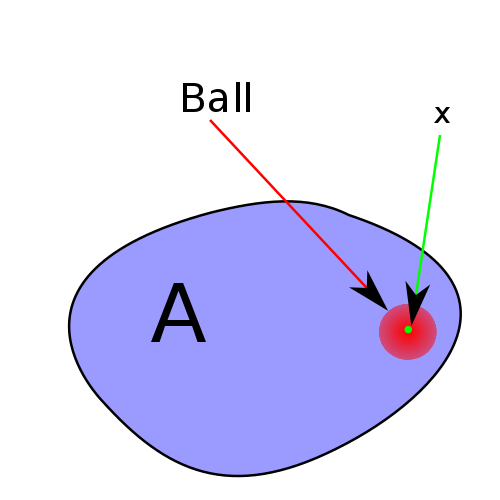
\includegraphics[width=0.45\textwidth]{img/openset}
      \caption{Quelle: Wikipedia}
\end{figure}


 \end{frame}


\begin{frame}
    \frametitle{Stochastik}
\framesubtitle{Lebesgue Maß}

    \begin{block}{Hüllquader}
Für eine Menge $A \subset \mathbb{R}^n$ bezeichnen wir eine Menge von Quadern $\{ I_j \; | \;  I_j \in \mathbf{I}(n)  \}$ mit $A \subset \bigcup_j I_j$ als Hüllquader für $A$.
\end{block}

    \begin{block}{ Lebesguesche äußere Maß}
Für eine Menge $A \subset \mathbb{R}^n$ definieren wir das Lebesguesche äußere Maß durch 
\begin{align*}
\mu (A):=   \inf \biggl \{ \sum_{j=1}^{\infty}   \text{vol} (I_j)\; ; \; I_j \in \mathbb{I}(n); A \subset \bigcup_{j= 1}^{\infty} I_j \biggr \} 
\end{align*}
\end{block}
    \begin{block}{Infimum}
Größte untere Schranke.
\end{block}
 \end{frame}

\begin{frame}
    \frametitle{Angewandte Mathematik}

\begin{figure}[H]
      \centering
    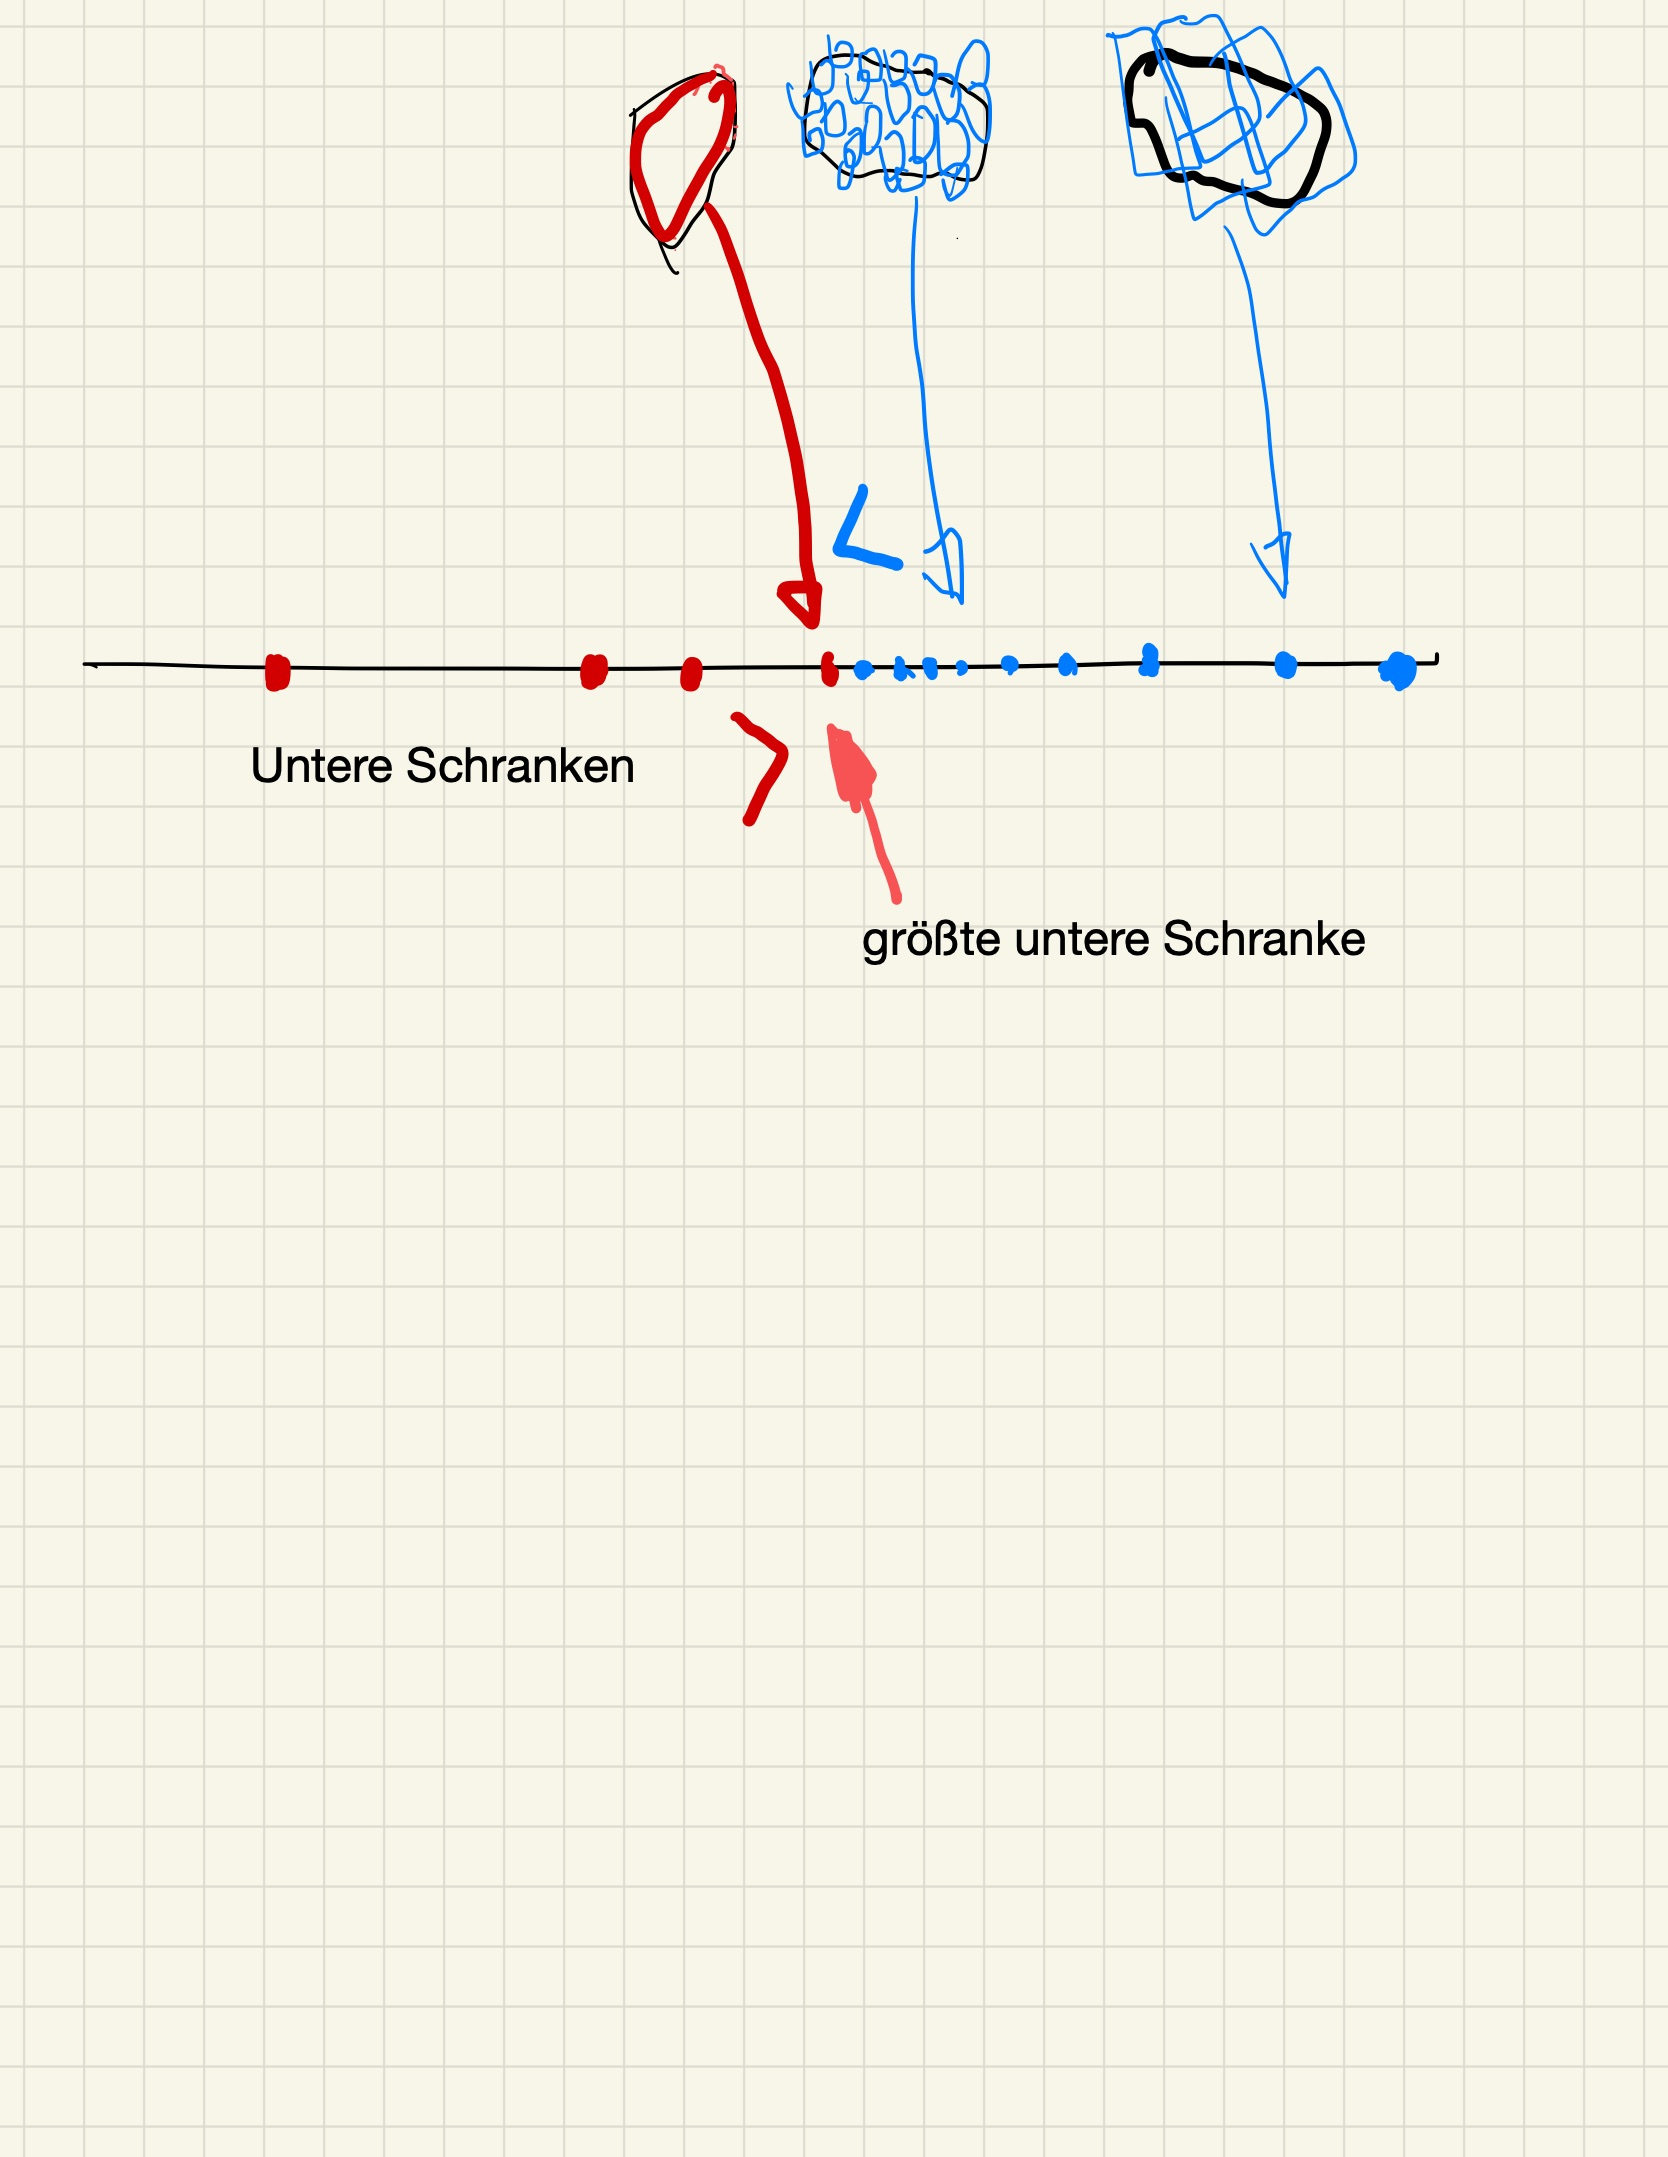
\includegraphics[width=0.8 \textwidth]{img/untereschranke}
      \caption{}
\end{figure}
 \end{frame}



\begin{frame}
    \frametitle{Stochastik}
\framesubtitle{Lebesgue Maß}
    \begin{block}{Monotonie}
Für $A \subset B \subset \mathbb{R}^n$ ist $\mu(A) \leq \mu(B)$.
\end{block}

    \begin{block}{Beweis}
Da $A \subset B$ Teilmenge ist, sind Hüllquader von $B$  auch Hüllquader von $A$ und damit  $\mu(A) \leq \mu(B)$.
\end{block}
 \end{frame}


\begin{frame}
    \frametitle{Stochastik}
\framesubtitle{Lebesgue Maß}
    \begin{block}{$\sigma$-subadditivität}
Sei $A_j \subset \mathbb{R}^n$ eine Folge von Mengen. Dann gilt
\begin{align*}
\mu (\bigcup_j^{\infty} A_j ) \leq \sum_{i=1}^{\infty} \mu(A_j)
\end{align*}
\end{block}
 \end{frame}


\begin{frame}
    \frametitle{Stochastik}
\framesubtitle{Lebesgue Maß}
    \begin{block}{Beweis}
Für jedes $A_j$ und $\epsilon > 0$ können wir  eine geeignete Überdeckung  $A_j \subset \bigcup_k  K_{j,k}$ mit Hüllquadern $K_{j,k}$ finden, so dass 
 $\sum_k \text{vol} (K_{j,k}) \leq \mu(A_j) + \frac{\epsilon}{2^{j+1}}$.
Da $ \bigcup_j A_j \subset \bigcup_j \bigcup_k  K_{j,k}$ eine Überdeckung mit Hüllquadern ist, folgt
\begin{align*}
\mu \biggl (  \bigcup A_j  \biggr) & \leq \sum_j \sum_k \text{vol} (K_{j,k}) \leq  \bigl( \sum_j  \mu(A_j) + \frac{\epsilon}{2^{j+1}} \bigr)  \\
&= \bigl (\sum_j \mu(A_j) \bigr ) + \epsilon
\end{align*}
(Die letzte Gleichung beruht auf dem Wert der \href{https://de.wikipedia.org/wiki/Geometrische_Reihe}{geometrischen Reihe}).
Da die letzte Aussage für beliebiges $\epsilon > 0$ gilt, folgt die Behauptung.
\end{block}
 \end{frame}



\begin{frame}
    \frametitle{Stochastik}
\framesubtitle{Meßbare Mengen}
    \begin{block}{Meßbare Menge}
Für einen Quader $I$ gilt $\mu(I) =  \text{vol}(I) $.
\end{block}
 \end{frame}

 \begin{frame}
    \frametitle{Stochastik}
\framesubtitle{Meßbare Mengen}
Da $I$ eine Überdeckung von $I$ mit Hüllquadern ist, folgt $\mu(I) \leq \text{vol}(I)$.
\\ Müssen also noch $\mu(I) \geq \text{vol}(I)$ zeigen: \\
Dazu Sei $I' := \{ I_k \}_k$ eine abzählbare überdeckung von $I$ mit Hüllquadern.
Vergrößere die Quader $I_k$ etwas, so dass man $I_k^*$ erhält mit 
$I_k \subset \overset{\circ}{I_k^*}$ und $\text{vol}(I_k^*) \leq (1+ \epsilon)\text{vol}(I_k)$.
\\
Da $I$ kompakt ist (beschränkt und abgeschlossen), gibt es eine endliche Auswahl mit 
$$I \subset \bigcup_{i=1}^n I_i^*$$
\end{frame}


\begin{frame}
    \frametitle{Stochastik}
\framesubtitle{Meßbare Mengen}
Damit erhlten wir
\begin{align*}
    \text{vol}(I) & \leq \sum_{i=1}^n  \text{vol}(I_i^*) \\
& (1 + \epsilon) \sum_{i=1}^n  \text{vol}(I_i) \\
& \leq (1 + \epsilon) \sum_{i=1}^{\infty}  \text{vol}(I_i) \\
 & = (1 + \epsilon) \mu(S)
\end{align*}

\end{frame}



\begin{frame}
    \frametitle{Stochastik}
\framesubtitle{Meßbare Mengen}
    \begin{block}{Maßproblem}
Es gibt disjunkte Mengen  $A,B \in \mathcal{P}(\mathbb{R}^n)$ mit $\mu(A \cup B) \neq \mu(A) + \mu(B)$. Konstruiert werde diese mit Hilfe der 
\href{https://www.youtube.com/watch?v=SJ8YoV6YZFA}{Vitali Mengen}. Hierfür wird das Auswahlaxiom benötigt.
\end{block}

    \begin{block}{Lösung}
$\mu$ Einschränken auf "kleinere" $\sigma$-Algebren.
\end{block}

 \end{frame}


\begin{frame}
    \frametitle{Stochastik}
\framesubtitle{Meßbare Mengen}
    \begin{block}{Meßbare Menge}
Eine Menge $A$ heißt Lebesgue meßbar, wenn für alle $Q \subset \mathbb{R}^n$
\begin{align*}
\mu(Q) = \mu(Q \cap A) + \mu(Q \cap A^c)  
\end{align*}
gilt. Die Menge der Lebesgue meßbaren Mengen wird mit $\mathcal{L}^n$ bezeichnet.
\end{block}


    \begin{block}{Meßbare Menge}
$\mathcal{L}^n$ ist eine $\sigma$-Algebra und für  zwei Lebesgue meßbare Mengen  $A,B \in \mathcal{L}^n$ ist
\begin{align*}
 \mu(A \cup B) = \mu(A) + \mu(B)
\end{align*}

\end{block}

 \end{frame}


 \begin{frame}
    \frametitle{Stochastik}
\framesubtitle{Meßbare Mengen}
Aufgrund der $\sigma$-subadditivität gilt immer
$$ \mu(Q) = \mu(Q \cap A \cup Q \cap A^c) \leq \mu(Q \cap A) +  \mu(Q \cap A^c) $$
Um zu zeigen, dass eine Menge mesßbar ist, reicht es also zu zeigen, dass 
$$\mu(Q)  \geq \mu(Q \cap A) +  \mu(Q \cap A^c) $$
gilt.
\end{frame}



\begin{frame}
    \frametitle{Stochastik}
\framesubtitle{Meßbare Mengen}
$\mathcal{L}^n$ ist eine $\sigma$-Algebra: \\
Ist $A$ messbar, so ist $A^c$ messbar, da die Bedingung symmetrisch ist in $A$ und $A^c$. \\
Sind $A, B \in \mathcal{L}^n$ messbar, so gilt 
\begin{align*}
    \mu(Q)  & \geq \mu(Q \cap A) +  \mu(Q \cap A^c) \\
    & \geq \mu(Q \cap A ) + \mu(Q \cap A^c  \cap B) + \mu(Q \cap A^c  \cap B^c) \\
    & [\text{Messbarkeit von B angew. auf $Q\cap A^c$}] \\
    & \geq \mu((Q \cap A)  \cup (Q \cap A^c  \cap B)) + \mu(Q \cap A^c  \cap B^c) \\
    & [\text{$\sigma$-subadditivität}] \\
= & \mu(Q \cap (A \cup B))+  \mu(Q \cap (A \cup B)^c) 
\end{align*}
\; \; \; \; \; \; \; \; [\href{https://de.wikipedia.org/wiki/Mengenlehre}{Mengenlehre}]    
\end{frame}

\begin{frame}
    \frametitle{Stochastik}
\framesubtitle{Meßbare Mengen}
$\sigma$-additivität: \\
Für $M,N \in \mathcal{L}^n$ mit $M \cap N = \emptyset$ folgt aus Meßbarkeitsbedingung für $Q' = Q \cap (M \cup N)$
$$ \mu (Q \cap (M \cup N)) = \mu (Q \cap M) +  \mu (Q \cap N)$$
und via Induktion für eine Folge disjunkter, messbarer Mengen $A_j$
$$ \mu (Q \cap (\bigcup_j A_j)) = \sum_j \mu (Q \cap A_j)$$

\end{frame}



\begin{frame}
    \frametitle{Stochastik}
\framesubtitle{Meßbare Mengen}
$\sigma$-additivität: \\
Wir erhalten 
\begin{align*}
    \mu(Q) & \geq \mu(Q \cap (\bigcup_j A_j)) + \mu(Q \cap (\bigcup_j A_j)^c) \\
    & \geq \sum_j \mu(Q \cap A_j) + \mu(Q \cap A_j^c) \\
    & \geq \mu(Q \cap A) + \mu(Q \cap A^c) \\
    & \text{[$\sigma$-subadditivität]}
\end{align*}
\end{frame}





 \begin{frame}
    \frametitle{Stochastik}
\framesubtitle{Meßbare Mengen}

    \begin{block}{Meßbare Menge}
        Offene Mengen sind meßbar.
\end{block}

\end{frame}

 \begin{frame}
    \frametitle{Stochastik}
\framesubtitle{Meßbare Mengen}
Wir zeigen: Jede offene Menge $U$ ist abzählbare Vereinigung nicht überlappender Quader. 

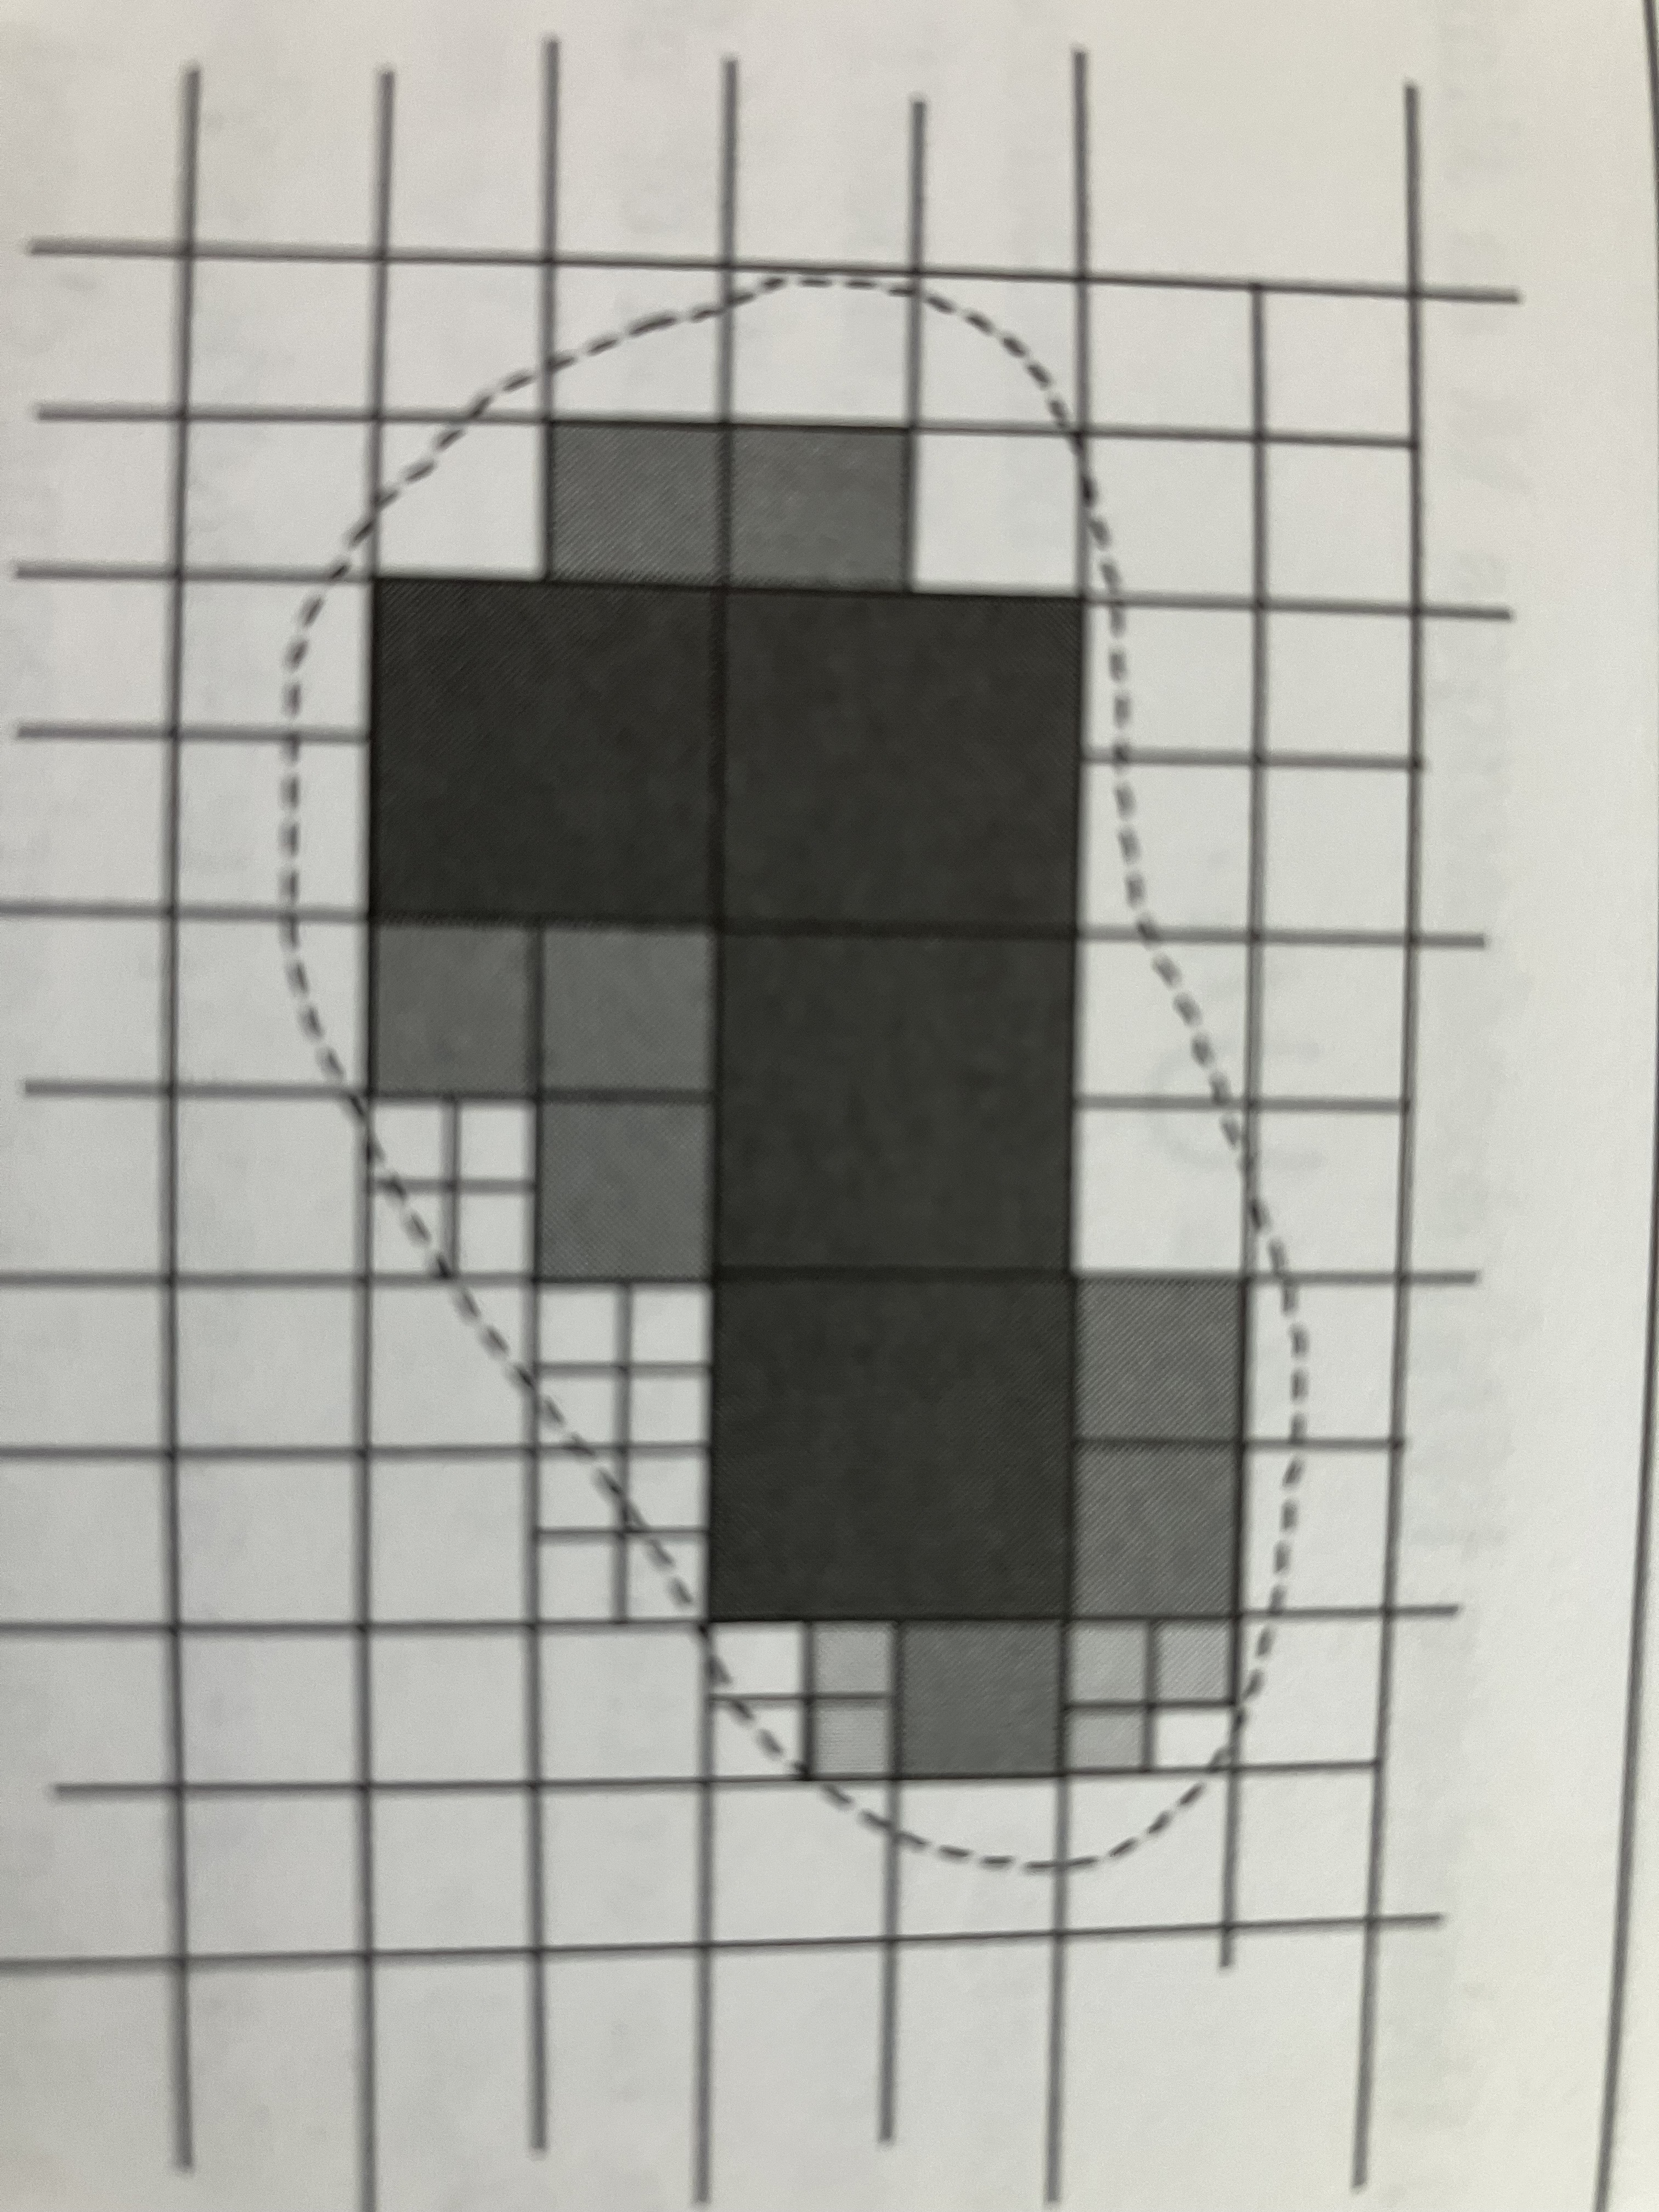
\includegraphics[scale=0.04]{img/openmeasurable.jpg}
 \end{frame}


\begin{frame}
    \frametitle{Stochastik}
\framesubtitle{Meßbare Mengen}

\begin{block}{Meßbare Menge}
Eine Menge $A$ ist genau dann Lebesgue meßbar, 
wenn es für bel. $\epsilon > 0$ 
eine abgeschlossene Menge $C$ und eine offene Menge $U$ gibt 
mit $C \subset A \subset U$ und 
$\mu (U \setminus C ) < \epsilon $
\end{block}

 \end{frame}

\begin{frame}
    \frametitle{Zufallsvariablen}
\framesubtitle{}

\begin{block}{Borel'sche Sigma-Algebra}
Die Borel'sche   $\sigma$-Algebra $\mathcal{B}(\mathbb{R}^n)$über $\mathbb{R}^n$ ist die kleinste  $\sigma$-Algebra, die alle offenen Mengen $\mathcal{U}$ enthält, also 
\begin{align*}
A_\sigma (\mathcal{U}) := \bigcap \{  \mathcal{A} \subset \mathcal{P}(\mathbb{R}^n);  \;   \mathcal{U}  \subset  \mathcal{A},  \;  \mathcal{A} \text{ ist $\sigma$-Algebra} \}
\end{align*}
\end{block}

\begin{block}{Existenz}
Die Borel'sche   $\sigma$-Algebra existiert, da die Potenzmenge eine   $\sigma$-Algebra ist.
\end{block}
\begin{block}{Messbarkeit}
    Die Borel'sche   $\sigma$-Algebra ist in der $\sigma$-Algebra der Lebesgue messbaren Mengen enthalten.
    \end{block}
 \end{frame}



\end{document}

